\documentclass[border=2pt]{standalone}
\usepackage{pgfplots}
\usetikzlibrary{arrows.meta}
\pgfplotsset{compat=1.18}
\begin{document}
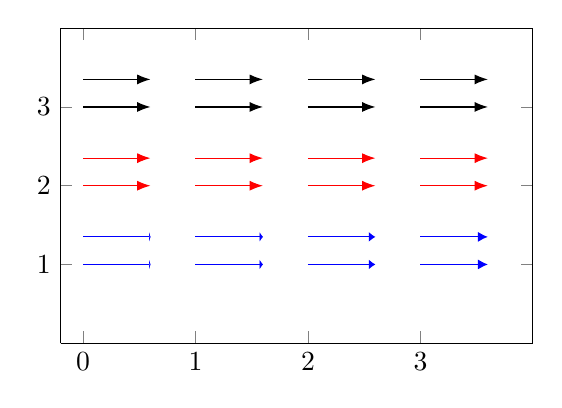
\begin{tikzpicture}
\begin{axis}[view={0}{90},scale only axis,width=6cm,height=4cm,
  xmin=-.2,xmax=4,ymin=0,ymax=4,zmin=-1,zmax=1,enlargelimits=false,
  domain=0:3,samples=4,samples y=2,xtick={0,1,2,3},ytick={1,2,3},point meta rel=per plot]
  \addplot3[blue,point meta=x,point meta min=0,point meta max=4,y domain=1:1.35,
    quiver={u=.6,v=0,every arrow/.append style={
      -{Latex[scale length={max(.1,\pgfplotspointmetatransformed/1000)}]}}}] {0};
  \addplot3[red,point meta=x,y domain=2:2.35,
    quiver={u=.6,v=0,every arrow/.style={-{Latex}}}] {0};
  \addplot3[black,y domain=3:3.35,quiver={u=.6,v=0,
    every arrow/.style={-{Latex[scale length={max(.1,\pgfplotspointmetatransformed/1000)}]}}}] {0};
\end{axis}
\end{tikzpicture}
\end{document}
